\documentclass{IEEEtran}
\usepackage[utf8]{inputenc}
\usepackage[spanish]{babel}
\usepackage{graphicx}
\usepackage{rotating}

\usepackage{todonotes}

\usepackage[backend=biber]{biblatex}
\addbibresource{bibliography.bib}

\title{RTOS en placa de desarrollo EDU-CIAA para el control de un accionamiento electromecánico básico}
\author{Gonzalo Gabriel Fernández}
\date{\today}

\begin{document}

\maketitle

\begin{abstract}
    Proyecto final de la cátedra Microcontroladores y Electrónica de Potencia de la Facultad de Ingeniería de la Universidad Nacional de Cuyo. Consiste en el diseño e implementación de un sistema embebido para el control de un accionamiento electromecánico básico, basado en el sistema operativo de tiempo real FreeRTOS, sobre la placa de desarrollo EDU-CIAA-NXP del proyecto CIAA. El principal objetivo del proyecto es la implementación y puesta en práctica de todas las características fundamentales del RTOS.
\end{abstract}

\section{Introducción}
El objetivo del trabajo es la implementación de una aplicación basada en el sistema operativo de tiempo real freeRTOS, sobre la placa de desarrollo EDU-CIAA, para el control de un sistema electromecánico básico que tiene como fin únicamente la demostración visual de lo que sucede en la electrónica. Se busca implementar todos los conceptos fundamentales de FreeRTOS, basándose en el libro \textit{Mastering the FreeRTOS Real Time Kernel}\cite{FreeRTOS}, por más que algunos de estos conceptos tengan una aplicación forzada y se alejen de lo práctico o lo más conveniente. Esto es porque la principal finalidad del proyecto es aprender a utilizar FreeRTOS por sobre obtener un controlador del sistema con buen criterio de diseño y eficiente.

Además, el proyecto también busca una introducción al flujo de trabajo del proyecto CIAA (Computadora Industrial Abierta Argentina). Salvo algunas excepciones, no se profundizó en la programación de los microcontroladores a nivel de registros, sino que se utilizó la capa de abstracción proveída por las librerías sAPI y LPCOpen, incluidas en el firmware de dicho proyecto CIAA.

\section{Aplicaciones de tiempo real}
Previo al planteo de la elección de un sistema operativo de tiempo real como base en el diseño de una determinada aplicación, es importante definir cuándo una aplicación es ``de tiempo real''. Se dice que una aplicación es de tiempo real cuando posee características tales que en su ejecución debe cumplir distintos requisitos de tiempo. Es decir, el diseñador debe garantizar que ciertos eventos se desarrollarán dentro de un margen de tiempo establecido.

Ese margen de tiempo puede ser más estricto o más flexible según cuál sea la aplicación en específico, y las características impuestas por el desarrollador. Para establecer una medida de la ``importancia'' o rigidez que tienen esos tiempos, surgen los conceptos de requisitos de tiempo tipo \textit{soft} (o su traducción al español como suave o blando) y requisitos de tiempo tipo \textit{hard} (o su traducción al español como duro). Toda la bibliografía consultada concuerda en que los requisitos de tiempo \textit{soft} son aquellos que, de no cumplirse su tiempo límite especificado, tiene como consecuencia una disminución en la \textbf{calidad} del desempeño de la aplicación. Por el otro lado, los requisitos de tiempo \textit{hard} son aquellos que, de no respetar dicho margen de tiempo, resulta en una falla del sistema.

Para clarificar la diferencia entre requisitos duros y blandos, ciertas fuentes suelen colocar ejemplos como navegación autónoma, marcapasos o instrumentación médica sensible, es decir, aplicaciones donde una falla es realmente crítica, como aplicaciones de tiempo real duro; y otros ejemplos donde solo se afecta la calidad, como servicios de chat y similares, como aplicaciones de tiempo real blando. Al realizar este trabajo, una de las conclusiones es que este tipo de ejemplos generan confusión, ya que quién se esta introduciendo en el concepto puede confundir la medida de qué tan duro es un requisito de tiempo con una medida de severidad de la falla de un sistema. 

Lo principal a tener en cuenta es que en última instancia, ante un determinado comportamiento de un sistema, quien establece el límite entre disminución en la calidad de desempeño y una falla es el diseñador. También es importante que, en general, no es todo el sistema el que posee estas restricciones de tiempo, sino un determinado aspecto en particular. Para resaltar esto, se puede utilizar como ejemplo el proyecto llevado a cabo, donde los motores deben moverse a posiciones definidas en un determinado lapso de tiempo (esto establece la velocidad de los motores), por lo que esa es una característica del sistema que requiere tiempo real; mientras que, por ejemplo, no tiene relevancia en qué momento en específico se expone el valor de posición del motor en un display (en otra aplicación diferente esto si puede llegar a ser una característica que en el diseño se contemple como de tiempo real duro).

En definitiva, una aplicación es de tiempo real si como diseñador se debe garantizar que ciertas funcionalidades del sistema se ejecutan en determinados instantes de tiempo. Si al diseñar un sistema, se poseen diferentes procesos en los que el tiempo directamente no es una variable relevante y se ejecutarán cuando el procesador este disponible, entonces el requisito de tiempo real es nulo y no es necesario considerar una plataforma que soporte tiempo real. 

\section{Sistemas Operativos de Tiempo Real}
Un sistema operativo con la característica de \textbf{tiempo real} es entonces aquel cuya estructura está diseñada para cumplir requisitos de tiempo. Estos sistemas brindan todas las ventajas de un sistema operativo convencional: el programa ahora se plantea en diversos hilos que se ejecutarán en pseudo paralelismo, prácticamente independientes entre sí. Esto hace que la aplicación sea más fácil de mantener y escalar, favorece la modularidad del sistema, la tarea de desarrollo es más sencilla si esta involucrada más de una persona, mayor reutilización de código, mayor eficiencia (si la aplicación es lo suficientemente compleja como para justificar un RTOS), testing más sencillo, etc. Incluso se dispone del \textit{Idle} que básicamente es el proceso ejecutado en el tiempo muerto, que puede utilizarse para distintos fines como bajo consumo, medir tiempo libre, diferentes chequeos, etc.

Específicamente la característica de tiempo real del sistema operativo genera una capa de abstracción donde el desarrollador puede despreocuparse (hasta cierto punto) del orden de ejecución del programa, utilizando las API relacionadas con la sincronización en el tiempo de los distintos procesos. Esto marca la principal diferencia con los sistemas embebidos sin sistema operativo, donde la programación sigue un esquema de ``super loop'' y cada aspecto de cómo se desenvuelve la aplicación en el tiempo es bien definido. En sistemas simples esto no es un problema, pero en sistemas complejos, la opción más sencilla puede ser el uso de un RTOS donde se plantean diferentes procesos por separado y el sistema operativo se encarga de cuál ocupa el procesador en cada instante.

\subsection{FreeRTOS}
FreeRTOS es una de la varias opciones de sistemas operativos de tiempo real de código abierto. Su objetivo es ser simple y pequeño, es desarrollado y mantenido por \textit{Real Time Engineers Ltd.}. Es distribuido bajo licencia MIT, y la amplia lista de arquitecturas que soporta es uno de los motivos por el cual es tan popular.

\section{Computadora Industrial Abierta Argentina}
La \textbf{Computadora Industrial Abierta Argentina} (CIAA) es un proyecto que nace en el año 2013 como una iniciativa conjunta entre el sector académico y el industrial de Argentina.

La primera versión de la CIAA es denominada CIAA-NXP, por estar basada en un procesador de la empresa \textit{NXP Semiconductors}. Luego se desarrollaron otras versiones basadas en procesadores de otras marcas, como la CIAA-FSL, la CIAA-INTEL, la CIAA-PIC, etc. Esto convierte a la CIAA no solo en la primer y única computadora \textbf{industrial} y \textbf{abierta}, sino también en la primera realmente \textbf{libre}, ya que su diseño no está atado a los procesadores de una determinada compañía.

Además, se diseñó una versión educativa de la plataforma, denominada \textbf{EDU-CIAA}, más simple y de menor costo, para lograr un impacto en la enseñanza primaria, secundaria y universitaria.

\subsection{Placa de desarrollo EDU-CIAA-NXP}
La EDU-CIAA-NXP (figura \ref{fig:edu-ciaa}) es entonces, una versión de bajo costo de la CIAA-NXP y es la utilizada para este proyecto.

\begin{figure}[ht]
    \centering
    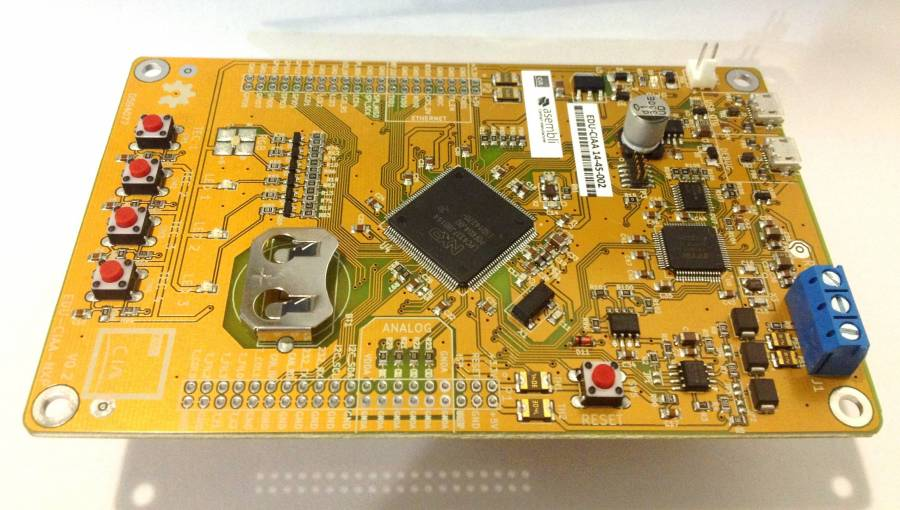
\includegraphics[width=0.45\textwidth]{../edu_ciaa.jpg}
    \caption{Placa de desarrollo EDU-CIAA-NXP.}
    \label{fig:edu-ciaa}
\end{figure}

Su microcontrolador es el LPC4337 (dual core ARM Cortex-M4F y Cortex-M0). La placa también cuenta con los siguientes módulos:

\begin{itemize}
    \item 2 puertos micro-USB (uno para aplicaciones y debugging, otro para alimentación).
    \item 4 salidas digitales implementadas con leds RGB.
    \item 4 entradas digitales con pulsadores.
    \item 1 puerto de comunicaciones RS 485 con bornera.
    \item 2 conectores de expansión:
    \begin{itemize}
        \item P1:
        \begin{itemize}
            \item 3 entradas analógicas (ADC0, 1, 2 y 3),
            \item 1 salida analógica (DAC0),
            \item 1 puerto I2C,
            \item 1 puerto asincrónico full duplex (para RS-232).
            \item 1 puerto CAN,
            \item 1 conexión para un teclado de 3x4,
        \end{itemize}
        \item P2:
        \begin{itemize}
            \item 1 puerto Ethernet,
            \item 1 puerto SPI,
            \item 1 puerto para Display LCD con 4 bits de datos, Enable y RS.
            \item 9 pines genéricos de I/O.
        \end{itemize}
    \end{itemize}
\end{itemize}

En la figura \ref{fig:edu-ciaa-modulos} se presenta un diagrama de bloques con los módulos que posee la placa.

\begin{figure}
    \centering
    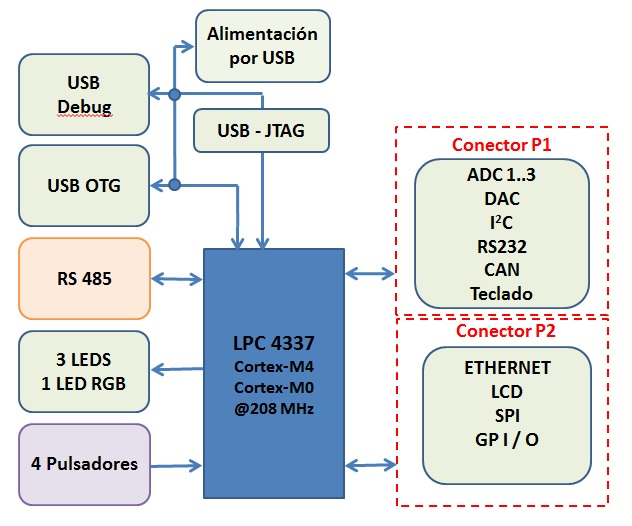
\includegraphics[width=0.45\textwidth]{../modulos_edu_ciaa.jpg}
    \caption{Diagrama de bloques con módulos de placa EDU-CIAA-NXP}
    \label{fig:edu-ciaa-modulos}
\end{figure}

\section{Accionamiento electromecánico: brazo robótico paralelo básico}
Para reflejar de una forma concreta las acciones ejecutadas en la electrónica del sistema, se optó por implementar el control de un brazo robótico paralelo básico. Su tamaño es reducido, ya que solo tiene un fin educacional, y por lo tanto los actuadores son sencillos y de poca potencia. El robot implementado es denominado EEZYBOTARM MK3, publicado por EEZYrobots y diseñado por Carlo Franciscone. 

\begin{figure}[ht]
    \centering
    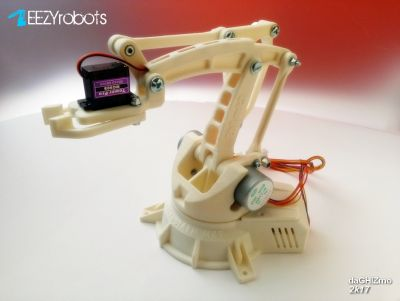
\includegraphics[width=0.45\textwidth]{../robot_arm.jpg}
    \caption{Brazo robótico paralelo EEZYBOTARM MK3 de EEZYrobots, diseñado por Carlo Franciscone.}
    \label{fig:robot-arm}
\end{figure}

Los actuadores del robot consisten en tres motores paso a paso monopolares 28BYJ-48 con drivers ULN2003, y su extremo operativo es accionado por un servo motor Tower Pro SG90.

Además del brazo robótico con sus tres motores paso a paso y servo motor, la aplicación también tiene un display donde se observará la información del estado en que se encuentra el brazo. Las consignas que recibirán los motores será a través de protocola UART desde PC o mediante un encoder rotativo. Como accesorio secundario en la aplicación se encuentran los LEDs de la placa EDU-CIAA como indicadores visuales y un buzzer como indicador auditivo.

\section{Componentes fundamentales de FreeRTOS}
A continuación se describe brevemente los diferentes componentes escenciales de FreeRTOS según el libro \textit{Mastering the FreeRTOS Real Time Kernel}, y su uso dentro de la aplicación.

\subsection{Asignación de memoria dinámica}
El proceso de asignación de memoria dinámica (asignación de memoria en tiempo de ejecución) es un aspecto muy importante en FreeRTOS, ya que es el modo en que el sistema asigna RAM cada vez que un objeto del kernel es creado.

El lenguaje C tiene dos funciones en la librería estándar para este tipo de asignación de memoria: \textit{malloc()} y \textit{free()}, para asignar y liberar memoria respectivamente. Algunos inconvenientes al usar este tipo de funciones son:

\begin{itemize}
    \item Su implementación no suele ser pequeña para un sistema embebido.
    \item No suelen ser \textit{thread-safe}, es decir que no se asegura que al llamarlas no se esta modificando o leyendo recursos compartidos.
    \item No son determinísticas. Dos llamados diferentes tomarán tiempos de ejecución diferentes.
    \item Pueden provocar fragmentación.
\end{itemize}

Es por esto que FreeRTOS brinda como APIs públicas \textit{pvPortMalloc()} y \textit{vPortFree()}, que tienen el mismo prototipo que sus equivalentes de la librería estándar de C. En el proyecto se utilizan, por ejemplo, al asignar memoria para los mensajes recibidos. Memoria que luego de ser procesado el mensaje es liberada.
\todo[inline]{TO DO: Problemas con la utilización de vPortFree()}

Debido a que se utiliza asignación de memoria dinámica en el proyecto, es importante estudiar los 5 tipos de pilas de memoria que brinda FreeRTOS como ejemplos de esquemas de asignación:

\begin{itemize}
    \item \textit{Heap 1}: Implementación básica de \textit{pvPortMalloc()} y sin implementación de \textit{vPortFree()}. Se utiliza en aplicaciones que nunca eliminan tareas ni otro tipos de objetos de kernel. Es el caso de este proyecto, sin embargo se mencionó el uso de un buffer de mensajes que si son dinámicos (cabe aclarar que es algo que puede evitarse, sin embargo se lo implementa como un caso de aplicación).
    \item \textit{Heap 2}: Esquema que solo se mantiene por compatibilidad, pero no se recomienda utilizar.
    \item \textit{Heap 3}: Utiliza las funciones de la librería estándar de C \textit{malloc()} y \textit{free()}.
    \item \textit{Heap 4}: A diferencia del 3, combina bloques de memoria libre en un bloque de mayor tamaño, y utiliza un algoritmo de \textit{first fit} (se asigna el primer bloque libre con espacio suficiente), lo que previene la defragmentación.
    \item \textit{Heap 5}: La única diferencia con el 4, es que no esta limitado a la asignación de memoria partiendo de un único array asignado estáticamente.
\end{itemize}

En el proyecto se optó por utilizar un esquema \textit{heap 4}.

\subsection{Tareas}
Las tareas son básicamente funciones implementadas en C y son programas en sí mismas. Su estructura es similar a la de una función \textit{main()} típica en sistemas embebidos, con un bucle que debe ejecutarse de forma infinita. Cada tarea se ejecuta de forma independiente en \textit{pseudoparalelismo}, y al crearse se les asigna automáticamente su propia pila de memoria.

Sus estados principales son \textit{running} y \textit{not running}, cuando el procesador esta ejecutando el código de la tarea y cuando no, respectivamente. El estado \textit{not running} puede expandirse, y podemos decir que una tarea se puede encontrar en una de las siguientes situaciones:

\begin{itemize}
    \item Bloqueada: La tarea se encuentra esperando un determinado evento.
    \item Suspendida: No están disponibles para el \textit{scheduler}.
    \item Lista: Ya esta disponible para pasar a estado \textit{running}, pero todavía no es seleccionada por el \textit{scheduler}.
\end{itemize}

El cambio de estado en una tarea es únicamente dirigido por el \textit{scheduler} de FreeRTOS. Para definir cuál tarea tiene más importancia de ejecución sobre otra, existe el concepcto de prioridad: cuándo el \textit{scheduler} deba decidir cuál es la próxima tarea a colocar en estado \textit{running} deberá observar cuál es la de mayor prioridad.

Para seleccionar esa próxima tarea a ejecutar, el \textit{scheduler} se ejecuta mediante una interrupción periódica denominada \textit{tick interrupt}. En el proyecto la frecuencia de dicha interrupción es de 1000Hz.

No es necesario expecificar un ejemplo de tarea ya que se utilizan en prácticamente todos los aspectos del trabajo.

\subsection{Algoritmos de \textit{scheduler}}
El algoritmo del \textit{scheduler} es el que decidirá que tarea ejecutará de entre la lista de tareas en estado listas o \textit{ready}.

El tipo de algoritmo a utilizar se configura con dos variables: uso de \textbf{preemption} y uso de \textbf{time slicing}:

\begin{itemize}
    \item \textit{Scheduling de prioridad fija pre-emptive con time slicing}: Ambas variables en 1. No cambia la prioridad de las tareas (si pueden cambiarse su prioridad las tareas mismas), inmediatamente se hace ``pre-empt'' de la tarea en estado \textit{running} si otra de mayor prioridad entra en estado \textit{ready} (esto quiere decir que el scheduler automáticamente en el \textit{tick} le dará el procesador a la tarea de mayor prioridad en estado \textit{ready}), y el \textit{time slicing} indica que a tareas de igual prioridad en estado \textit{ready} se les brindará el procesador alternadamente en intervalos de tiempo iguales (esos intervalos de tiempo son iguales a dos interrupciones por tick).
    \item \textit{Scheduling de prioridad fija pre-emptive sin time slicing}: \textit{time slicing} en 0. En este caso al no haber \textit{time slicing}, cuando tareas de igual prioridad se encuentren en estado \textit{ready}, solo habrá cambio de contexto (el \textit{scheduler} asigna el procesador a una tarea diferente) cuando la tarea en estado \textit{running} se bloquee o se suspenda o haya \textit{pre-empt} de una tarea de prioridad mayor.
    \item \textit{Scheduling cooperativo}: \textit{preemption} en 0 y \textit{time slicing} en cualquier valor. Solo hay cambio de contexto cuando la tarea en estado \textit{running} se bloquee o suspenda, o cuando explícitamente hace un \textit{yield} (solicitar explícitamente la entrada del \textit{scheduler}).
\end{itemize}

En este trabajo se optó por utilizar un algoritmo de \textit{scheduling} de prioridad fija pre-emptive con time slicing.

\subsection{Queues o colas}
Las colas brindan un mecanismo de comunicación tarea a tarea, tarea a interrupción e interrupción a tarea. Normalmente se utilizan como buffers FIFO (\textit{First Input First Output}). FreeRTOS implementa colas por copia y no por referencia, ya que estas presentan ventajas y en última instancia pueden utilizarse como colas por referencia guardando punteros.

Las características principales de esta estructura son las siguientes:

\begin{itemize}
    \item Pueden ser accedidas por cualquier número de tareas o rutinas de interrupción.
    \item Se puede especificar un tiempo de bloqueo de una tarea si intentó leer una cola y ésta se encontraba vacía.
    \item También puede especificarse un tiempo de bloqueo de una tarea si intentó escribir en una cola y ésta se encontraba completa.
    \item Se pueden agrupar de forma que una tarea quede bloqueada hasta que alguna del grupo se encuentre disponible para su lectura o escritura.
\end{itemize}

En el proyecto se utilizaron colas de recepción y transmisión que contienen los caracteres recibidos o ha ser enviados por UART, y también colas con elementos de tamaño variable como lo son la cola de mensajes recibidos y la cola de consignas de los motores (ver figuras \ref{fig:diagrama-uart} y \ref{fig:diagrama-stepper}).

Si una tarea recibe información desde múltiples fuentes (esto aplica tanto a colas como a semáforos), FreeRTOS nos permite agrupar esas fuentes en \textit{sets}. Estos \textit{sets} evitan que la tarea deba hacer un polling en turnos de las fuentes.

Un ejemplo de la aplicación de \textit{sets} se implementó en la comunicación de pulsos del encoder a la tarea de control de dicho componente. Allí se implementaron dos semáforos contadores, ambos con pulsos, que se diferencian en la dirección enviada (ver figura \ref{fig:diagrama-encoder}).

\subsection{Mailbox}
El mailbox dentro de los RTOS es una estructura de datos que permite guardar información a ser leída por múltiples tareas o interrupciones. FreeRTOS no hace diferencia entre un mailbox y una cola de longitud unitaria. En lugar de implementar una nueva estructura con diferente funcionamiento a una cola, lo que brinda son dos APIs que permiten adaptar las colas al funcionamiento de un mailbox.

Estas dos APIs son \textit{xQueueOverwrite()} que permite sobrescribir el elemento de información en la cola (de hecho solo debe utilizarse en colas con longitud uno), y \textit{xQueuePeek()} que permite realizar la lectura sin eliminar el dato de la cola (que es lo que sucedería ante una acción de \textit{Receive}).

Un ejemplo de mailbox se encuentra en la selección del motor a modificar con el pulsador del encoder rotativo (ver figura \ref{fig:diagrama-encoder}).

\subsection{Timers por software}
\label{sec:software-timer}
Los timers por software se utilizan para planificar la ejecución de una función en un determinado tiempo en el futuro, o a intervalos regulares a una frecuencia fija. Al ser por software no requieren de hardware, y son implementados completamente por el RTOS.

Existen dos tipos:
\begin{itemize}
    \item De un disparo: Donde una vez ejecutada la función de \textit{callback} deben resetearse manualmente.
    \item De recarga automática: Se resetean automáticamente por lo que la función de \textit{callback} se ejecutará periódicamente.
\end{itemize}

Se dice que los timers tienen dos estados: \textit{running} cuando expiran y ejecutan una función de \textit{callback} y dormidos el resto del tiempo.

Todas las funciones de \textit{callback} de los timers por software se ejecutan en el contexto de la misma tarea \textit{daemon} del RTOS. Esta tarea se crea automáticamente al lanzar el \textit{scheduler}, por eso se le denomina \textit{daemon}, haciendo referencia a un proceso que permanece de forma continua a lo largo de toda la ejecución del programa.

Esto es importante, ya que entonces no se debe utilizar APIs dentro de las funciones de \textit{callback} que puedan generar un cambio de contexto, es decir, que bloqueen el RTOS \textit{daemon}. Por ejemplo, se puede llamar \textit{xQueueReceive()} pero solo si el parámetro \textit{xTicksToWait} esta seteado en 0.

En el proyecto hay tres instancias de timers por software, y son los encargados del movimiento de los motores paso a paso (ver figura \ref{fig:diagrama-stepper}).

\subsection{Uso de FreeRTOS desde una rutina de interrupción}
Dado que muchas veces es necesario el uso de funcionalidades del RTOS dentro de una rutina de interrupción, y teniendo en cuenta que al ejecutarse una rutina de interrupción estamos saliendo del control del sistema operativo en tiempo real, FreeRTOS provee una versión de las APIs convencionales pero para ser ejecutadas en estas circunstancias. Todas aquellas APIs terminadas en ``FromISR'' son de este tipo.

Por este mismo motivo es muy aconsejable que las rutinas de interrupción sean cortas, y que si es necesario realizar un procesamiento considerable, dirigirlo a una tarea para que lo realice y finalizar la rutina de interrupción. Para sincronizar las interrupciones con las tareas que ejecutarán el procesamiento vinculado a ellas, se utilizan objetos como semáforos y colas.

En el proyecto se utilizaron APIs de FreeRTOS dentro de rutinas de interrupción como las de UART o las de entradas/salidas de propósito general utilizadas por el encoder (ver figuras \ref{fig:diagrama-uart} y \ref{fig:diagrama-encoder}).

\subsection{Semáforos}
Los semáforos son objetos de comunicación que permiten la sincronización entre interrupciones y tareas, aunque su uso no se restringe solamente a éste. Su funcionamiento consiste en bloquear a la tarea hasta que desde la interrupción se realice la acción de ``dar'' el semáforo y la tarea pueda ``tomarlo''.

La descripción anterior es la de un semáforo binario, pero también existen los semáforos contadores que son equivalentes a colas con una longitud mayor a uno. La tarea que lee dicho semáforo no esta interesada en la información que contiene, sino en la cantidad de elementos. Cada vez que se ``da'' al semáforo se agrega un elemento, y cada vez que se ``toma'' del semáforo se elimina un elemento.

En el proyecto se utilizó dos semáforos contadores en la implementación del encoder, donde ambos acumulan los pulsos que se reciben (ver figura \ref{fig:diagrama-encoder}).

\subsection{Gestión de recursos y mutex}
Un problema que hay que tener en cuenta en sistemas multitarea como el de este proyecto, es la posibilidad de que una tarea acceda a un recurso compartido y sea expulsada del estado \textit{Running} antes de completar ese acceso. Si esto ocurre, mientras la tarea se encuentra en este estado, otra tarea que comparta el mismo recurso puede acceder y modificarlo, resultando en una corrupción de datos.

Una forma de mantener y asegurar la consistencia de datos es a través de la técnica de \textbf{exclusión mutua}. El objetivo es que una vez que una tarea accede a un recurso compartido, ninguna otra puede acceder hasta que ese recurso haya vuelto a un estado de consistencia, o lo que es lo mismo, esté disponible para volver a ser accedido. De esta forma, las tareas tienen acceso exclusivo soble dicho recurso.

El objeto que permite poner en práctica la técnica de exclusión mutua es el \textit{mutex}. Básicamente consiste en un tipo de semáforo binario para controlar el acceso a un recurso. Al acceder a un recurso compartido la tarea tomará el \textit{mutex}, y ningun otro proceso podra acceder hasta que ese \textit{mutex} no sea ``devuelto''.

Algo a tener en cuenta al utilizar este recurso, es el fenómeno de \textbf{inversión de prioridad}. La inversión de prioridad sucede cuando una tarea de baja prioridad toma el \textit{mutex} y luego otra de alta prioridad intenta acceder al mismo recurso y, por lo tanto, se bloquea esperando su liberación. Si antes de que la tarea de baja prioridad libere el \textit{mutex}, una tercera tarea de prioridad media (prioridad mayor que la de baja prioridad pero menor que la de alta prioridad) hace un \textit{pre-empt}, el resultado es que la tarea de prioridad alta no solo tiene que esperar a la tarea de prioridad baja, sino también a la de prioridad media. Para disminuir el impacto de este fenómeno, los \textit{mutex} se diferencian de los semáforos convencionales en su característica de \textbf{prioridad heredada}. Básicamente se aumenta temporalmente la prioridad de la tarea que toma el \textit{mutex}, y de esta forma las tareas como la de prioridad media en el ejemplo anterior no realizan el \textit{pre-empt} sobre la tarea que tomó dicho \textit{mutex}.

En el proyecto se aplicaron \textit{mutex} para la protección de la cola de transmisión por UART y para la cola de consignas de motores.

Otra forma muy efectiva de garantizar la exclusión mutua de un recurso, son las tareas \textit{gatekeeper}. Basicamente consiste en una tarea convencional que tiene el control total sobre el recurso a proteger, cualquier otro proceso que necesite el acceso lo deberá hacer indirectamente a través de los servicios que brinde la tarea \textit{gatekeeper}. 

En el proyecto se utilizaron dos de este tipo de tareas a la hora de implementar la comunicación UART: una encargada de la transmisión de datos y otra del procesamiento de la información recibida.

\subsection{Notificación de tareas}
Las notificaciones de tarea proporcionan una forma de comunicación entre tareas (o tareas y rutinas de interrupción) sin la necesidad de un objeto de comunicación, como lo son las colas, semáforos y grupos de eventos. Esto permite que la comunicación sea directa.

Algunas limitaciones de las notificaciones de tareas son:

\begin{itemize}
    \item Solo se puede notificar a una única tarea.
    \item No se puede acumular múltiples elementos con información.
    \item Bloquear un proceso hasta que el envío sea válido. Si se envía una notificación a una tarea que ya tenía una notificación pendiente, no se puede esperar en estado bloqueado a que la tarea resetee su estado de notificación.
\end{itemize}

Implementación de notificaciones de tarea sencillas en el proyecto pueden encontrarse, por ejemplo, en el control de flujo de trabajo de los motores paso a paso. Allí, la función de \textit{callback} del timer, si encuentra que no hay pasos pendientes, envía una notificación a la tarea de control de los motores para que ésta inicialice la próxima consigna.

Un ejemplo de notificaciones más complejas, es la gestión de errores por notificación en la tarea de sincronización de mensajes. Allí cada bit del valor de notificación da la información de cuál fue el error en el mensaje recibido (ver figura \ref{fig:diagrama-app}).

\section{Implementación de los diferentes módulos del proyecto}
\label{sec:modulos}

A continuación se describe, mediante diagramas de flujo, el diseño e implementación de los diferentes módulos que conforman la aplicación.

\subsection{Comunicación UART}
\label{sec:uart}
Las colas permiten una forma sencilla de comunicación de interrupción a tarea, sin embargo hay que tener en cuenta que no es eficiente si la entrada de datos es a una frecuencia muy alta. En este proyecto se aplicó solo con fines de demostración, opciones más eficientes pueden ser el uso de DMA (\textit{Direct Memory Access}) o procesar todo dentro de la rutina de interrupción.

En la figura \ref{fig:diagrama-uart} puede observarse tanto el diagrama de transmisión como de recepción de mensajes por UART.

\begin{figure*}[ht]
    \centering
    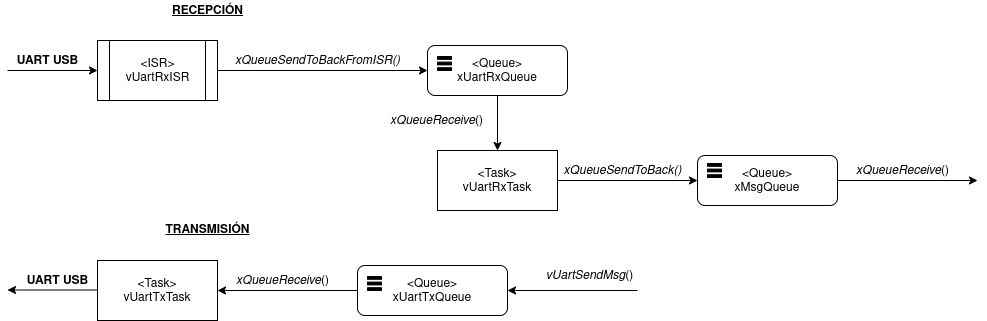
\includegraphics[scale=0.5]{../diagrama_uart.png}
    \caption{Implementación de comunicación UART con colas.}
    \label{fig:diagrama-uart}
\end{figure*}

La transmisión es muy sencilla: consiste en una tarea que realiza la lectura de una cola de mensajes pendientes a enviar, para luego efectivamente enviarlos por UART. Lo que se destaca es la protección de la cola a leer a través de un \textit{mutex}. Esto es así porque la escritura de la cola no es limitada a una única fuente, cualquier proceso que requiera enviar un mensaje puede acceder a ella.

Para la recepción de información se utilizan dos colas. La primera es escrita por la rutina de interrupción, y consiste en los caracteres recibidos. Dichos caracteres son leídos por la tarea encargada de ese procesamiento, asignándoles memoria como un único string que finaliza cuando se lee un final de línea. Una vez unido el mensaje en un único arreglo de caracteres, se envía a una segunda cola de mensajes recibidos.

\subsection{Control de motores paso a paso}
\label{sec:stepper}

En la figura \ref{fig:diagrama-stepper} puede observarse el diagrama de la implementación del control de motores paso a paso mediante el RTOS. Este módulo es, en comparación a los demás del proyecto, el más complejo y completo en cuanto a aplicación de funcionalidades de FreeRTOS.

\begin{figure*}[ht]
    \centering
    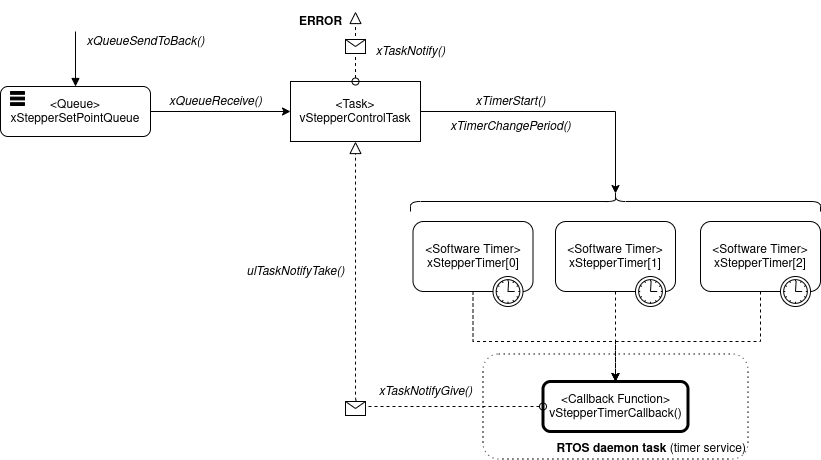
\includegraphics[scale=0.5]{../diagrama_stepper.png}
    \caption{Implementación de control de motores paso a paso.}
    \label{fig:diagrama-stepper}
\end{figure*}

El primer componente del módulo es una cola de los mensajes recibidos vinculados a la actividad de los motores. El tipo de elementos que guarda la cola son punteros a los mensajes (es un ejemplo de la utilización de colas para la comunicación de información de distintas dimensiones). Dado que dicha cola recibe información de múltiples fuentes, esta protegida mediante un \textit{mutex}.

Una tarea es la encargada de leer la información en la cola de consignas, que es escrita mediante acciones externas al módulo, y procesar el mensaje identificando los parámetros a setear: ID del motor, velocidad, posición y/o dirección. Una vez realizado ese procesamiento del mensaje, la tarea ejecuta una de las siguientes acciones:

\begin{itemize}
    \item Se devolverá un error si el mensaje es inválido, mediante el uso de notificación de tareas, seteando los bits correspondientes al error que se encontró.
    \item Se cambiará el período del timer indicado, para afectar la velocidad del motor.
    \item Se inicializa el timer indicado, con la información obtenida actualizada en su ID.
\end{itemize}

Probablemente los componentes más importantes del módulo son los timers por software. Habrá uno por cada motor (por lo tanto, tres) y en su ID se encuentra un puntero a la estructura que contiene la información del motor: pasos pendientes, dirección, identificación y estado del driver. Cada vez que los timers pasen a estado \textit{Running}, se ejecuta la función de \textit{callback} correspondiente. que decrementa la cantidad de pasos pendientes y actualiza el driver para afectar la posición del motor. 

Si la cantidad de pasos pendientes llega a cero, el timer se detiene a sí mismo y luego envía una notificación sencilla a la tarea de control de los motores, para que ésta pueda procesar la siguiente consigna en la cola y ejecutarla si es correcta. Es importante aclarar que el diseño planteado conduce a una ejecución de consignas de forma \textbf{secuencial}, es decir, nunca habrá más de un motor en movimiento a la vez.

Como se mencionó en la sección \ref{sec:software-timer}, la función de \textit{callback} de los timers se ejecuta en el contexto de la tarea \textit{daemon} del RTOS. Entonces, al \textit{daemon} se le asignó la prioridad más alta de la aplicación, ya que es imprescindible que los tiempos del timer se cumplan para un correcto funcionamiento de los motores.

\subsection{Encoder rotativo}
\label{sec:encoder}

En la figura \ref{fig:diagrama-encoder} se puede observar el diseño del módulo encargado de procesar la información recibida del encoder rotativo.

\begin{figure*}[ht]
    \centering
    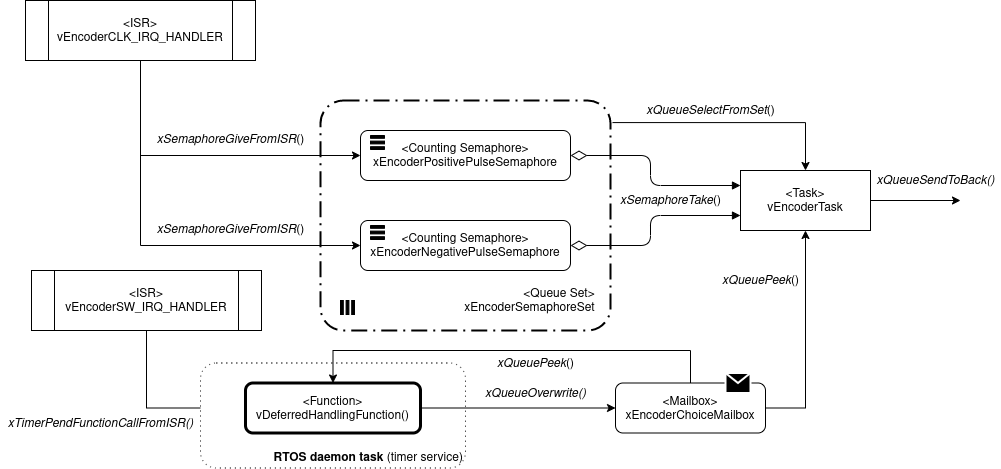
\includegraphics[scale=0.5]{../diagrama_encoder.png}
    \caption{Implementación de encoder rotativo como interfaz de usuario.}
    \label{fig:diagrama-encoder}
\end{figure*}

El rol del encoder en la aplicación es proveer una interfaz HMI muy simple que le permita al usuario seleccionar el motor a mover y moverlo. Para su lectura se deben manejar 3 entradas:

\begin{itemize}
    \item Una entrada de pulsador, que le permitirá al usuario cambiar de motor a mover.
    \item Una entrada de clock, que da los pulsos del movimiento de rotación del encoder. Cada pulso es equivalente a una consigna de un determinado ángulo.
    \item Una entrada de dirección, que al leerse junto con el pulso de clock recibido nos permite saber la dirección de rotación del encoder.
\end{itemize}

Entonces, el sistema recibe la interrupción tanto del pulsador como la señal de clock.

Ante el evento del pulsador, la rutina de interrupción incrementa el valor de un \textit{mailbox}. Este \textit{mailbox} guarda el motor elegido por el usuario.

Ante el evento del pulso de clock, se lee la entrada de dirección del encoder y según sea su valor 1 o 0 se agregara un ítem al semáforo contador de pulsos positivos o al semáforo contador de pulsos negativos respectivamente.

Una tarea es la encargada de procesar la información recibida. Dado que ambos semáforos contadores perteneces a un mismo \textit{set}, la tarea se bloquea esperando información en cualquiera de los dos semáforos. Al recibir un elemento en alguno de ellos, se construye el mensaje de consigna leyendo el motor seleccionado desde el mailbos, y se envía como un arreglo de caracteres a la cola de consignas pendientes.

\section{Interrupciones anidadas y particularidades de procesadores ARM Cortex-M}
El desafío más complejo en el desarrollo de la aplicación fue la implementación para que funcionen correctamente las rutinas de interrupción ejecutadas por el encoder rotativo (rutinas de interrupción ante flancos en pines GPIO).

Como ya se mencionó en la sección \ref{sec:encoder}, para la implementación del encoder además de las APIs de FreeRTOS se utilizó la librería LPCOpen, que brinda una capa de abstracción de más bajo nivel que la de la librería sAPI. Que sea de más bajo nivel da espacio a una mayor libertad en la configuración de las interrupciones, algo necesario para hacer la interrupción compatible con el RTOS.

Al plantear una configuración inicial de estas interrupciones con la librería LPCOpen, las rutinas de interrupción se ejecutaban correctamente a la hora de hacer parpadear un LED o imprimir un mensaje por UART, sin embargo a la hora de llamar una API de FreeRTOS cualquiera (terminada en ``FromISR'') el sistema fallaba dejando de funcionar.

En su libro, \textcite{FreeRTOS} menciona que es común confundir la prioridad de tareas en el FreeRTOS con la prioridad de interrupciones en el microcontrolador. También se aclara que es importante considerar que la relación entre el valor numérico de la prioridad y su valor lógico depende de la arquitectura del procesador.

Es importante, entonces, configurar la variable \textit{configMAX\_SYSCALL\_INTERRUPT\_PRIORITY} en aquellas plataformas que admitan el anidado de interrupciones, que es el caso del microcontrolador NXP LPC4337 en la placa EDU-CIAA. Dicha variable da la máxima prioridad \textbf{de interrupción} desde la cuál se puede llamar APIs de FreeRTOS.

Un modelo completo de anidado de interrupciones (donde todas las interrupciones pueden llamar APIs de FreeRTOS) se da cuando el valor de \textit{configMAX\_SYSCALL\_INTERRUPT\_PRIORITY} es seteada a un \textbf{valor lógico} mayor que \textit{configKERNEL\_INTERRUPT\_PRIORITY}. Esta última variable, da el valor de prioridad de la interrupción por tick y, por lo tanto, debe setearse al mínimo posible.

En los procesadores ARM Cortex-M, valores numéricos bajos de prioridad equivalen a valores lógicos altos de prioridad, es decir, una interrupción con valor 1 tiene mayor prioridad que otra con valor 5. Esto se presta especialmente a confusión, ya que en FreeRTOS la relación es la opuesta.

El controlador de interrupción de Cortex-M permite especificar la prioridad con un máximo de 8 bits, es decir, la prioridad de interrupción más baja posible será con valor numérico 255. Generalmente solo se implementa un subgrupo de esos 8 bits. De la librería CMSIS del microcontrolador LPC4337 se obtuvo que ese subgrupo es de 2 bits.

Con esta información, se encontraron dos posibles soluciones y ambas funcionan correctamente:

\begin{itemize}
    \item Setear mediante un llamado de LPCOpen la prioridad de NVIC de las interrupciones al mínimo (en el proyecto se las configuró en 255).
    \item Setear en la configuración de FreeRtos la variable \textit{configMAX\_SYSCALL\_INTERRUPT\_PRIORITY} a la prioridad máxima, es decir, a 1.
\end{itemize}

\section{Vinculación de los diferentes módulos de la aplicación}
\label{sec:vinculacion}

Una vez desarrollados los distintos módulos explicados en detalle en la sección \ref{sec:modulos}, se procedió a implementar su comunicación para poder cumplir el objetivo de mover el brazo robótico mediante consignas (ya sea por UART o a través del encoder rotativo).

Para esto, se implemento una última tarea que es la encargada de procesar los mensajes recibidos, enviarlos a los módulos que correspondan, y a su vez recibir los errores que estos mensajes puedan tener para poder comunicarlos por UART.

En la figura \ref{fig:diagrama-app} se puede observar la interconexión de todas las partes que conforman el proyecto.

\begin{sidewaysfigure*}[ht]
    \centering
    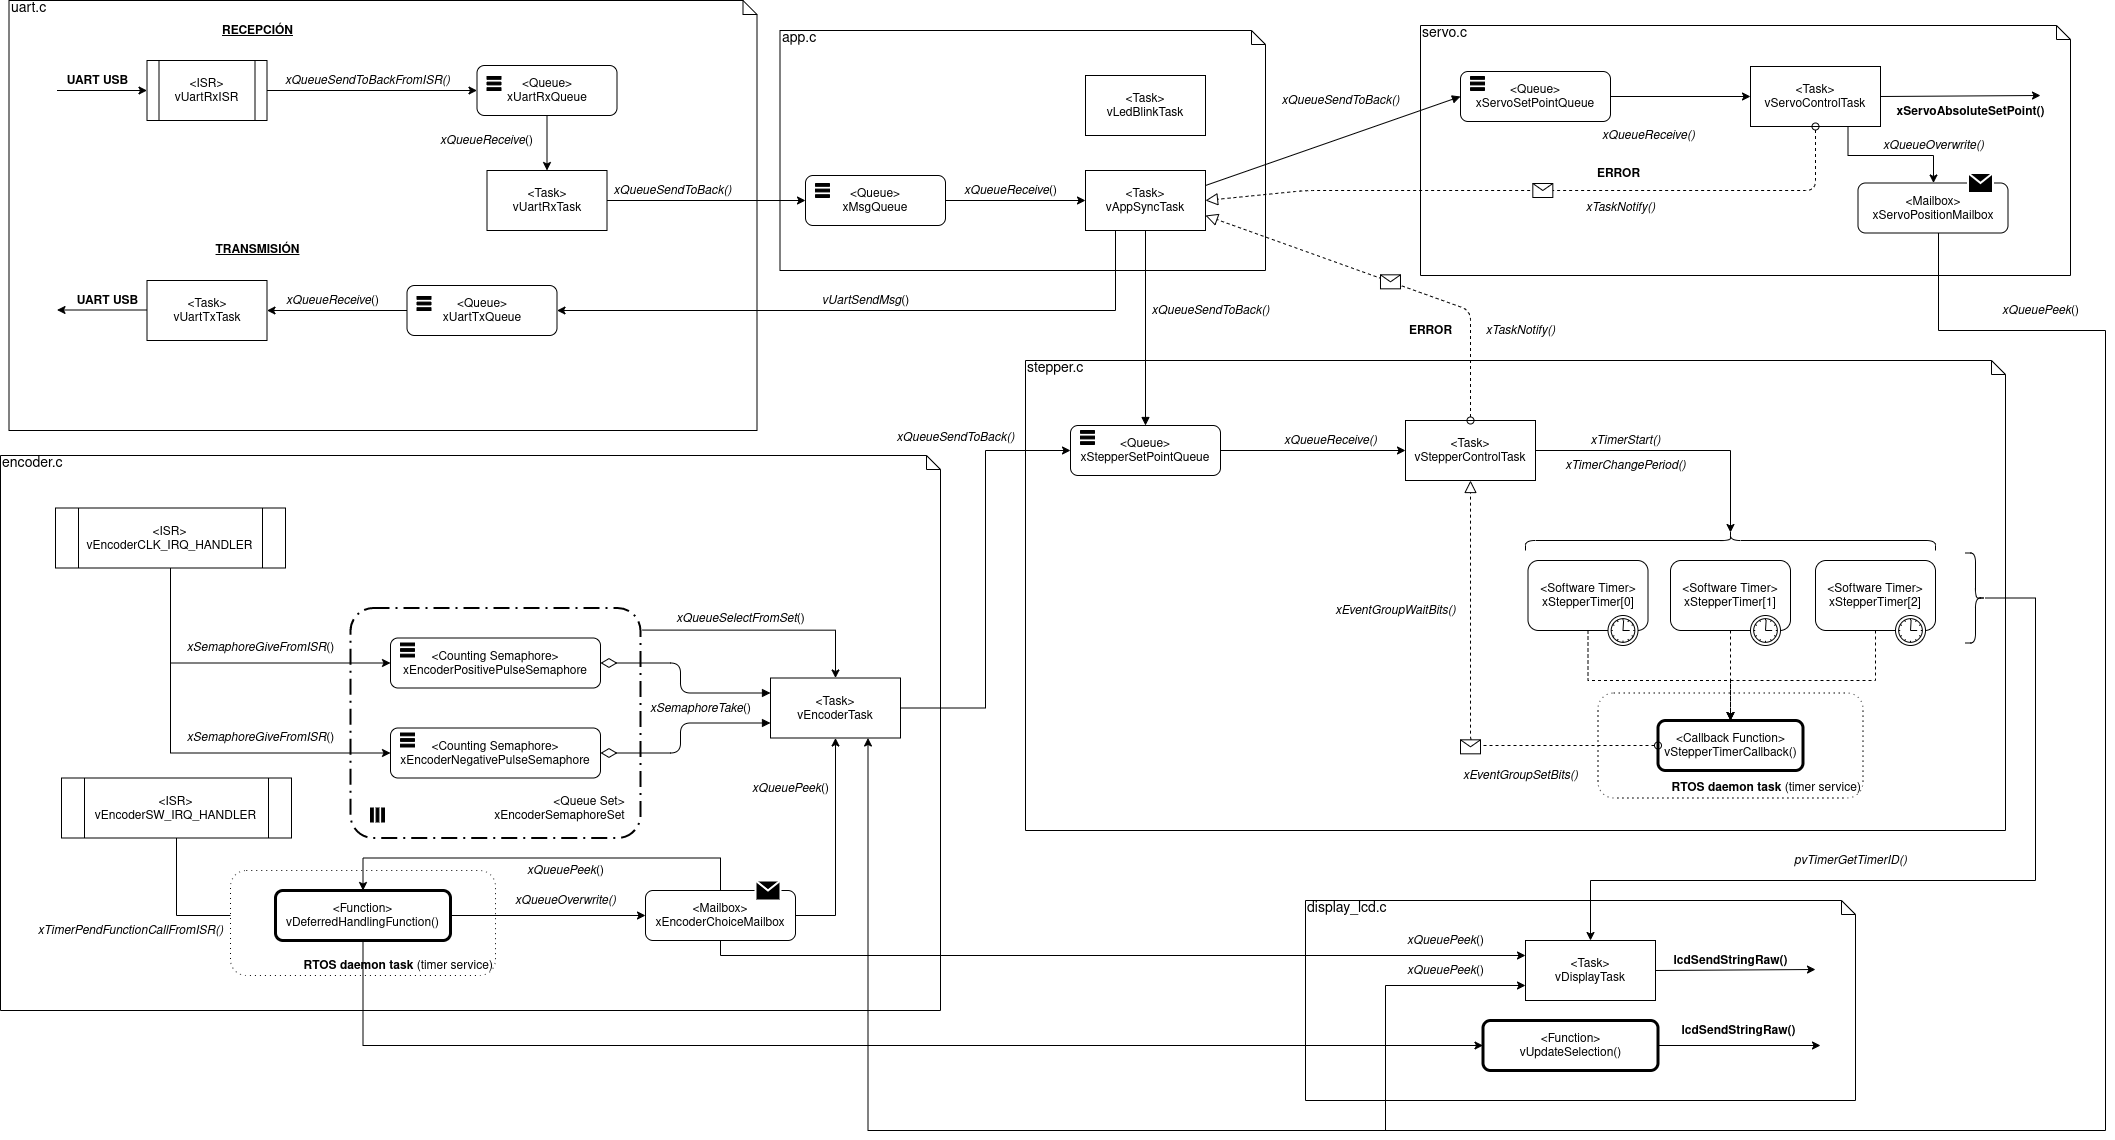
\includegraphics[scale=0.35]{../diagrama_app.png}
    \caption{Diagrama de interconexión de los diferentes módulos de la aplicación.}
    \label{fig:diagrama-app}
\end{sidewaysfigure*}

\section{Conclusiones}
\label{sec:conclusiones}
Todo el proyecto se desarrolló siguiendo el estilo de código propuesto por FreeRTOS, esto permitió programar de forma mucho más eficiente, estructurada y limpia. Además, para la documentación del código se siguieron los lineamientos del proyecto Doxygen, esto también hizo que el desarrollo del proyecto a medida que se iba complejizando fuera más sencillo de seguir.

Uno de los puntos a resaltar al finalizar el trabajo, es que aunque los diagramas parezcan complejos, el desarrollo de la aplicación no presenta dificultades si el diseño de la comunicación entre tareas esta bien planteada. Es muy sencillo seguir un diagrama e implementar todas los módulos con las APIs que provee el RTOS, trabajando sobre los procesos de forma independiente y llevando a cabo su intercomunicación hacia el final. La misma aplicación siguiendo un esquema de \textit{superloop} sería mucho más compleja de diseñar e implementar.

\section{Trabajo a futuro}
Analizar distintas herramientas de debugging para RTOS, como también estudiar en profundidad el desempeño que tiene el diseño implementado (tiempo en IDLE, cantidad de stack asignada a las diferentes tareas, etc.).

Fabricación de PCB donde poder montar todas las conexiones del hardware de forma más prolija (actualmente se encuentra en placa de prototipado).

\printbibliography

\end{document}